\documentclass[a4paper,12pt,twoside,dvipdfmx]{jreport} % A4 用紙,12pt フォント

% =========================== use package ================================== %
\usepackage[inner=25mm,outer=25mm,top=40mm,bottom=25mm]{geometry} % 余白の設定
\usepackage{titlesec} % 章タイトルのフォーマット
\usepackage{fancyhdr} % ヘッダーとフッターの設定
\usepackage{pdfpages} %pdf追加用

\usepackage[japanese]{babel} % 参考文献の表示を「参考文献」にする
\usepackage[T1]{fontspec} % 参考文献のコンパイルエラーを防ぐ. googlescholarからbibをコピペすると, OT1エンコーディングの文字コード「\k」が紛れ込むときがある. これがあると解析できなくてコンパイルエラーになる. それ対策

\renewcommand{\baselinestretch}{1.2} % 行間を1.2倍に設定
% ========================================================================== %

% ============================ header & footer ============================ %
\footskip=10mm % 文章からフッターまでの距離
\pagestyle{fancy}
\fancyhf{}
% 偶数ページの設定
\fancyhead[LE]{\leftmark} % 左ヘッダに章名
\fancyhead[CE]{}
\fancyhead[RE]{}
\fancyfoot[CE]{\thepage}

% 奇数ページの設定
\fancyhead[LO]{\rightmark} % 左ヘッダに節名
\fancyhead[CO]{}
\fancyhead[RO]{}
\fancyfoot[CO]{\thepage}
% ========================================================================== %


% ========================================================================== %
% 章タイトルを中央揃えに設定し、「第1章」の形式にする
\titleformat{\chapter}[display]
{\normalfont\huge\bfseries\centering} % フォントスタイルと中央揃え
{第\arabic{chapter}章}{20pt}{\Huge}
% ========================================================================== %


% ================================= title ================================== %
% \title{LaTeXでの文書作成入門ああああ}
% \author{おなまえたろう}
% \date{\today}
% ========================================================================== %


% ================================ document ================================ %
\begin{document}


% 表紙pdfの挿入
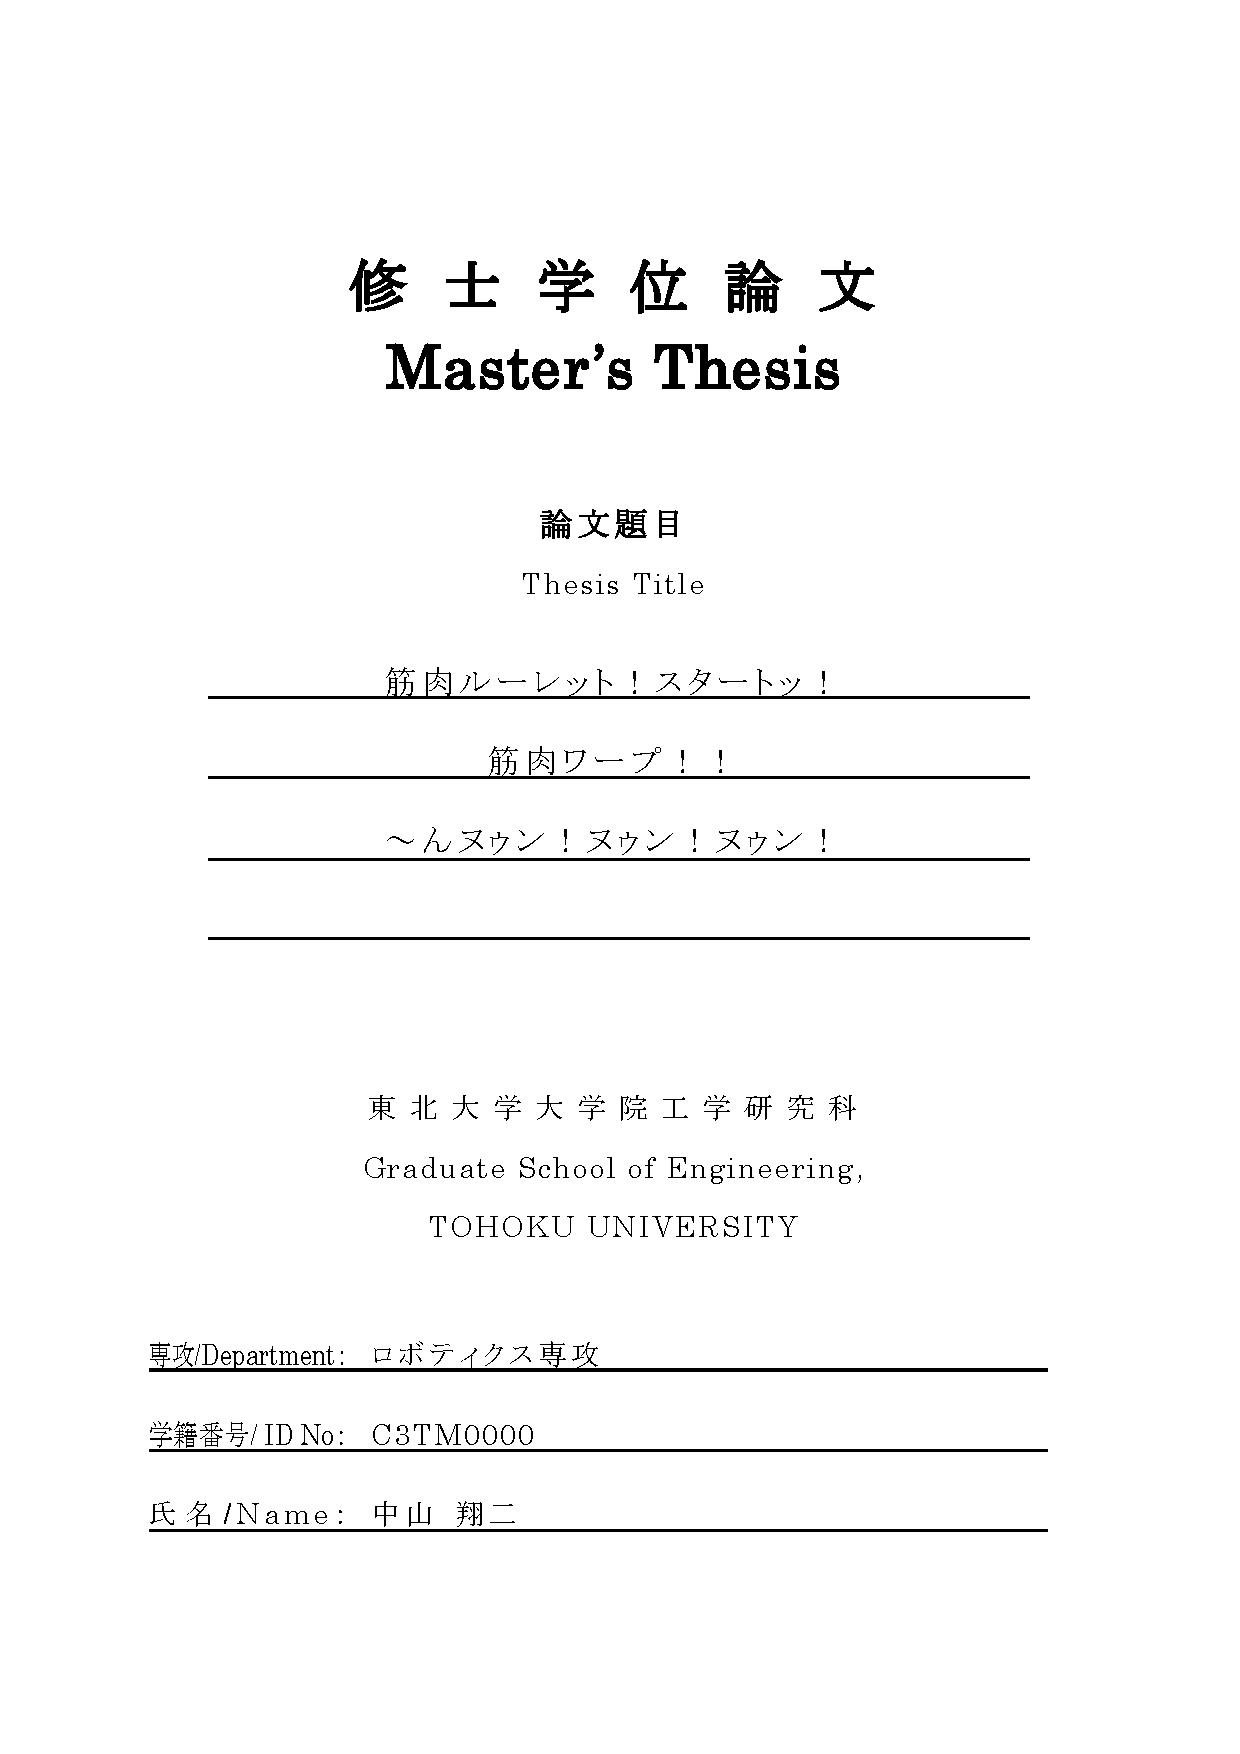
\includepdf[pages=-,fitpaper=true]{Other/hyoshi.pdf}
\cleardoublepage


% タイトル
\begin{titlepage}
    \begin{center}
  
        {\fontsize{24pt}{24pt}\selectfont  修士学位論文}
  
        \vspace{3cm}
  
        {\fontsize{20pt}{20pt}\selectfont \textbf{筋肉ルーレット!スタートッ!}}

        \vspace{0.5cm}
        {\fontsize{20pt}{20pt}\selectfont \textbf{筋肉ワープ!!}}

        \vspace{0.5cm}
        {\fontsize{20pt}{20pt}\selectfont \textbf{~んヌゥン!ヌゥン!ヌゥン!}}

        \vspace{5cm}
        {\fontsize{18pt}{18pt}\selectfont 令和6年度} 

        \vspace{0.5cm}
        {\fontsize{18pt}{18pt}\selectfont (令和7年?月??日 提出)} 
  
        \vspace{3cm}
        {\fontsize{18pt}{18pt}\selectfont 東北大学大学院工学研究科}

        \vspace{0.5cm}
        {\fontsize{18pt}{18pt}\selectfont ロボティクス専攻}
  
  
        \vspace{0.5cm}
        {\fontsize{18pt}{18pt}\selectfont 中山 翔二}
  
  
    \end{center}
  \end{titlepage}
\cleardoublepage


% 英語アブスト
\pagestyle{empty}

\begin{center}
    Muscle Roulette! Startt! Muscle Warp! ~Nnnnnn..! Nuun! Nuun!
\end{center}
\vspace{10mm}
\begin{center}
    Shoji Nakayama
\end{center}
\vspace{10mm}

\begin{center}
    Abstract
\end{center}
\vspace{10mm}

Nakayamakinnikun (September 17, 1978) is a Japanese male comedian, YouTuber, and bodybuilder. 
Born in Higashi Ward, Fukuoka City, Fukuoka Prefecture, he was a member of Yoshimoto Kogyo from 2000 to 2021 and freelance after 2022.
His real name is Shoji Nakayama.
He graduated from Wahirohigashi Elementary School in Fukuoka City, Wahirokaoka Junior High School in Fukuoka City, and Fukuoka Institute of Technology High School (now Joto High School attached to Fukuoka Institute of Technology).He had a muscular physique since his school days, but was more passionate about basketball than bodybuilding at that time.
He started muscle training at LBGYM in Kashii during his high school years.After becoming a TV personality, he visited LBGYM in 2005 and 2020 for a commercial TV program in Fukuoka.The program was aired on RKB Mainichi Broadcasting and TNC TV Nishinihon.
One of her classmates in high school was Motoei Kusakabe, a female judoist and bronze medalist at the Sydney Olympics.After graduating from high school, she entered Yoshimoto Sogo Gakuin (NSC) Osaka School as a 22nd year student [2][5].Before entering NSC, he appeared on the October 30, 1998 broadcast of Asahi Broadcasting Corporation's "Tantei!Night Scoop" on October 30, 1998 [Note 1] [Note 2].His classmates at NSC include Super Maradona, Kazunobu Kubota (Torosomon), and King Kong.After graduating from NSC in 2000, he debuted with Yoshimoto Kogyo as "Nakayamakini-kun," a pin comedian who performs gags using muscles[2].His godfather was Takayuki Haranishi (FUJIWARA), who was also his senior at NSC, but the name he initially invented was simply "Kinnikun" without "Nakayama." In 2001, he joined Yoshimoto Shinki Gekijou, where he played a clerk and a henchman of a yakuza gang.After completing a series of material in which he talks while using his muscular body to show off his muscles, he reports to his older brother (or employer, etc.), "I did all I had to do!I've done all I can do!"[Note 3] In January 2003, he won the judges' special award at the 24th ABC Comedy Newcomer Grand Prix.In 2006, he invented a new character, "Captain Bomber," who was supposed to be "a man from North Carolina who came to Japan to introduce American culture," and made it to the finals of the R-1 Grand Prix that same year.On this occasion, he placed a portrait of Nakayamakin on stage and performed his material as a different person from Kinnikun (even though he denied being called Kinnikun) [Note 4].When asked by his co-star Shinya Ueda (Kurimuchu) about his appearance on Asahi Broadcasting Corporation TV's "Gold Medal of Laughter" under the name Captain☆Bomber, he stubbornly denied that he was Nakayamakini-kun.In the Shinkigeki theater to which he belongs, he has been pushing "Captain Bomber" to the forefront and has started an event "Shinkigeki Bomber!He was also appointed as the image character of "Puururando RiO" at Misaki Park in Misaki Town, Sennan County, Osaka Prefecture, and his name recognition was greatly enhanced.Around the same time, he used his physical training to participate in the then-popular TBS "Who's the Strongest Man?The Fierce Muscle Battle!He has appeared in sports specials such as "The Sportsman No. 1 Championship" and has achieved a number of good results (see below).


\clearpage
\pagestyle{fancy} %abstract追加
\cleardoublepage


% 目次
\pagenumbering{roman} % ページ番号をローマ数字に設定
\setcounter{page}{1}
\tableofcontents % 目次を生成
\listoffigures %図目次
\listoftables %表目次


% 本文
\cleardoublepage % 奇数ページから始める
\pagenumbering{arabic} % ページ番号をアラビア数字に設定
\setcounter{page}{1} % ページ番号を1にリセット
\chapter{序論}
\section{四脚ロボット}
四脚ロボットのコントローラに関しては,様々なアプローチで研究がなされている.
代表的なアプローチとしては,モデルベースのコントローラ\cite{MIT_Cheetah_3,kim2019highly,sombolestan2021adaptive}や学習ベースのコントローラ\cite{tan2018simtoreal,Hwangbo_2019,kumar2021rma,challenging_terrain},バイオインスパイアのコントローラ\cite{Owaki1,Owaki2,4543306}などがある.
近年では,学習ベースのコントローラとバイオインスパイアのコントローラを組み合わせたアプローチ\cite{bellegarda2022cpgrl,cpgrl2,cpgrl3,Evolutionary}が注目されている.
本研究ではその一つであるCPG-RL\cite{bellegarda2022cpgrl}の不整地走破性能を向上させるため,姿勢反射機能を追加することを提案し,その性能の検証を行う.


\section{関連研究}
\subsection{モデルベースのコントローラ}
四脚ロボットのコントローラの一つにモデル予測制御(MPC)\cite{MIT_Cheetah_3,kim2019highly,sombolestan2021adaptive}に代表されるモデルベースのコントローラがある.
これらの研究では実機のロボットにおいて高い性能を示してきた.
しかし,これらの手法はオンライン最適化を行うため,モデルの精度への依存度が高く,緻密な設計が必要である.
また,事前に設計された足先の軌道やヒューリスティックな制御を用いるため,環境の変動に対する適応性が低い.
% Learning Based
\subsection{学習ベースのコントローラ}
一方,深層強化学習などを用いた学習ベースのコントローラは外乱や未知の環境に対してロバストな制御ポリシーを学習することが期待でき,注目を集めている.
近年の研究では、固有感覚のみを用いた「ブラインド」制御ポリシーの学習に成功しており,平地\cite{tan2018simtoreal,Hwangbo_2019}と不整地\cite{kumar2021rma,challenging_terrain,margolis2022walkwaystuningrobot}の両方での制御に成功している.
しかし,得られる動作が不自然であったり,報酬関数の設計が複雑になり,設計者のスキルへの依存が大きくなったりする.
それらを改善するために,実際の動物の運動データをエキスパートとして用いて模倣学習を行った研究\cite{RoboImitationPeng20}などもあるが,事前に膨大なエキスパートデータを必要とする.
% Biology Inspired
\subsection{バイオインスパイアのコントローラ}
また,四脚ロボットの歩行においては生物学から着想を得たバイオインスパイアのコントローラに関する研究も多く存在する.
特に脊椎動物の脊髄に存在する周期的な出力信号の協調パターンを生成する神経回路であるCPG(central pattern generator)に着想を得た研究が多い.
% このへんで改段落してCPGについての話題をまとめてもよさそうです。
CPGと単純な力フィードバックによって四脚ロボットの歩容の生成と遷移を可能にした研究\cite{Owaki1,Owaki2}やCPGにタッチセンサーからの感覚フィードバックを追加した研究\cite{4543306}などCPGを用いた手法はシンプルで汎用的である.
\section{問題点と既存の解決策}
Guillaumeらの研究\cite{bellegarda2022cpgrl}では深層強化学習に明示的にCPG (central pattern generator)を組み込んだ手法(以下CPG-RLと呼称)を用いて,通常の深層強化学習に比べてシンプルな報酬関数の設計で四脚ロボットの歩容を生成した.
CPGのフレームワークを用いて学習することで,学習の高速化とSim-to-Realの平易化を実現した.
また,全方向への移動が可能であり,ロボット質量の115%の13.75kgの荷重を動的に追加されても歩行を持続できるなど高いパフォーマンスを発揮した.
しかし,CPG-RL\cite{bellegarda2022cpgrl}では平地のみで学習を行っており,微小な段差へのロバスト性は示されているが,四脚ロボットが期待される不整地の歩行性能には届いていない.
脊椎動物は歩行や前足の配置をどのように調整するかを脊髄上部の領域で決定していること\cite{DREW201525}や代償的姿勢反応では脳幹網様体が関与していると\cite{doi:10.1152/jn.91013.2008}が知られており,姿勢を安定させ,不整地での十分な歩行性能を得るためにはCPGのみでなく,脊髄上部が担うとされる姿勢反射の機能が必要であると考える.
CPG-RLを用いて予期的な運動調整を行たった研究\cite{cpgrl2,cpgrl3}では,視覚情報を用いてCPG-RLのフレームワークで脚軌道中心のオフセットを調整し,ギャップのある地形での歩行を可能にした.

\section{研究目的}
そこで,本研究の目的は先行研究(CPG-RL)の不整地での歩行性能の向上とする.
初めに先行研究(CPG-RL)のフレームワークを用いて平地でCPG Policyの学習を行う.
続いて,学習したCPG Policyから計算される脚先の位置を調整するFoot Adjustment Policy を学習することで姿勢反射機能を追加する.
最後に不整地での歩行性能をベースラインと比較し,検証する.



\cleardoublepage % 奇数ページから始める
\chapter{手法}
\section{節のタイトル}
この文書はサンプルです.


\subsection{項のタイトル}
この文書はサンプルです.


\cleardoublepage % 奇数ページから始める
\chapter{結果}
\section{節のタイトル}
この文書はサンプルです.

\subsection{項のタイトル}
この文書はサンプルです.


% \cleardoublepage % 奇数ページから始める
\chapter{考察}
\section{節のタイトル}
この文書はサンプルです.

\subsection{項のタイトル}
この文書はサンプルです.


% \cleardoublepage % 奇数ページから始める
\chapter{結論}
\section{節のタイトル}
この文書はサンプルです.

\subsection{項のタイトル}
この文書はサンプルです.




% 謝辞
\cleardoublepage % 奇数ページから始める
\chapter*{謝辞}

\section*{}
本研究を行うにあたり,懇切丁寧なる御指導,御鞭撻を頂きました,指導教員の林部充宏教授に謹んで深く感謝の意を表します.
研究への取り組み方をはじめ,勉学以外の面においても,人として成長するために必要な多くのことを学ばせていただきました.

東北大学大学院医工学研究科医工学専攻の田中真美教授,東北大学大学院工学研究科ファインメカニクス専攻の山口健教授には,本論文をまとめるにあたって有意義な議論をさせていただきました.
深く感謝いたします.

ミーティングなどにおいて貴重な時間を割いていただき,本研究を行う過程で数々の有益な御助言をしていただいた大脇大准教授,沓澤京助教に深く感謝いたします.
同じシナジーをテーマとするグループとして日ごろから研究に関して様々な議論を交わし,相談に乗って頂いた松村拓海氏に心より深く感謝いたします.

研究グループの垣根を越えて議論を交わしていただいた,同期の古関駿介氏,轟将吾氏,利根川太氏,又吉康介氏,松本実南氏,Lucas Sulpice氏に心より深く感謝いたします.
研究以外の私生活に関する様々な相談に乗っていただき,大変有意義な二年間を送ることができました.

本研究を行うにあたり様々な面で大変お世話になりました,研究室の博士,学部の皆様,学会での議論に参加していただいた皆様に感謝いたします.

最後になりましたが,これまでの研究生活を温かく見守り,支えてくれた家族に,この場を借りて心より深く感謝いたします.

\begin{flushright}
2024年2月1日\\
おなまえ たろう
\end{flushright}



% 参考文献
\bibliographystyle{plain}
\bibliography{ref}


\end{document}
% ========================================================================== %